\pagestyle{empty}
\cleardoublepage
\pagestyle{fancy}
\chapter{Particionamento de domínios}\label{cap2}

Em Computação de Alto Desempenho é conhecido que para um bom algoritmo paralelo executar é preciso de uma boa estratégia para a divisão da entrada e a junção das várias soluções ao final. 

Além disso tem a preocupação com a alocação das tarefas entre os processadores levando em conta que ao final todos eles devem realizar uma quantidade de similar de processamento. Isso significa que a carga foi devidamente balanceada entre os processadores.

Nesse capítulo irei mostrar o que se tem feito nos últimos anos nessa área de subdivisão de domínios tentando focar nos pontos positivos e negativos de cada técnica que for apresentada.


%\section{Introdução}\label{cap2:intro}
\section{Particionamento Baseado no Centro de Densidade}

Em \cite{bib:Pirzadeh09} é descrito uma técnica baseada em Avanço de Fronteiras e Avanço de Camadas. Essa é uma técnica tridimensional mas pode ser adaptada para uma versão bidimensional.

Primeiramente é gerada a malha de superfície nos pontos dados como entrada, logo em seguida é feita uma estimativa de carga nos subdomínios utilizando uma \textit{octree}. Se necessário, serão criados planos de partições que dividem o domínio em regiões com cargas aproximadamente iguais. 

A posição destes planos são definidos através do centro de densidade da malha. Esse centro indica onde a massa efetiva do sistema está concentrada.

Em seguida, são identificadas as faces que interceptam o plano de partição e gera uma malha parcial na região do plano de corte. Depois disso, para cada lado da partição, são agrupadas as faces dos novos subdomínios. Esse processo é repetido até que um número máximo de subdivisões tenha ocorrido. Ao final da execução, tem que ser realizado uma junção de todos os segmentos das submalhas. A imagem~\ref{fig:imagem1} ilustra os principais passos dessa técnica.

 \begin{figure}[htbp]
     \centering
     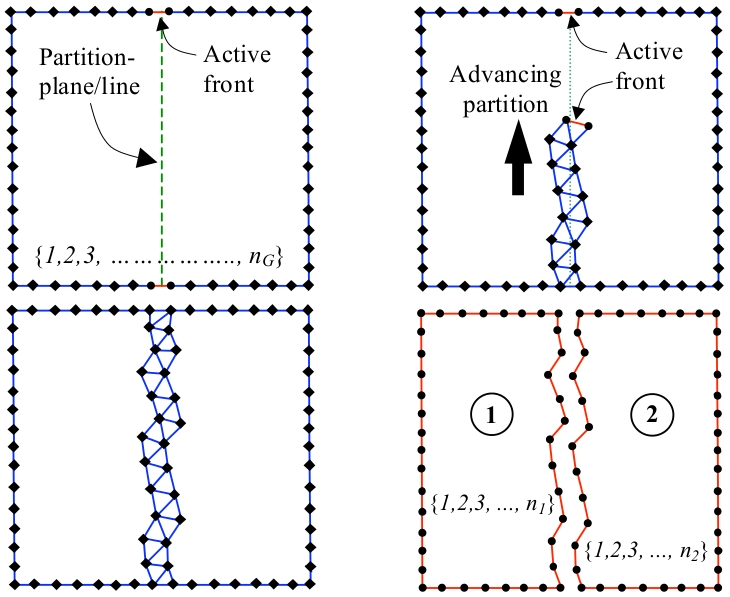
\includegraphics[width=0.8\textwidth]{imagem1}
     \caption{Os principais passos da técnica de \cite{bib:Pirzadeh09}.}
     \label{fig:imagem1}
 \end{figure}
 
 Como vantagens para essa técnica podemos citar que a utilização de avanço de camadas entre as partições faz com que a malha gerada seja praticamente idêntica a uma malha gerada sequencialmente. Ou seja, não será gerado padrões entre as partições do domínio. Outra vantagem é que não é necessário nenhum pré-processamento para definir ou construir as partições.

\section{Particionamento Baseado na Distância/Volume/Centro de Massa}
 
Em \cite{bib:Ivanov06} fizeram um algoritmo baseado em Delaunay em que o posicionamento do plano de corte é baseado no centro de massa e na matriz de inércia. O plano de corte é um plano perpendicular a um eixo que segue uma das três definições:

\begin{itemize}
  \item Planos criados são equidistantes;

  \item Volume entre os planos iguais;

  \item Passa pelo centro de massa;
\end{itemize}

A escolha de qual critério para criar os subdomínios vai depender da geometria da entrada. Dependendo da entrada um critério pode ser melhor que outro, qual escolher vai depender do conhecimento do usuário. Na imagem~\ref{fig:imagem2} as 3 formas de particionar são apresentadas.

Após ter o plano de corte definido é feita uma suavização da seção de corte e depois a sua triangularização, logo após é realizada a geração da malha nos subdomínios. Um problema bem visível nesse método é que para se ter um bom plano de corte é preciso ter um modelo com uma geometria bem comportada (sem forma côncava, alongada ou afinada).

 \begin{figure}[htbp]
     \centering
     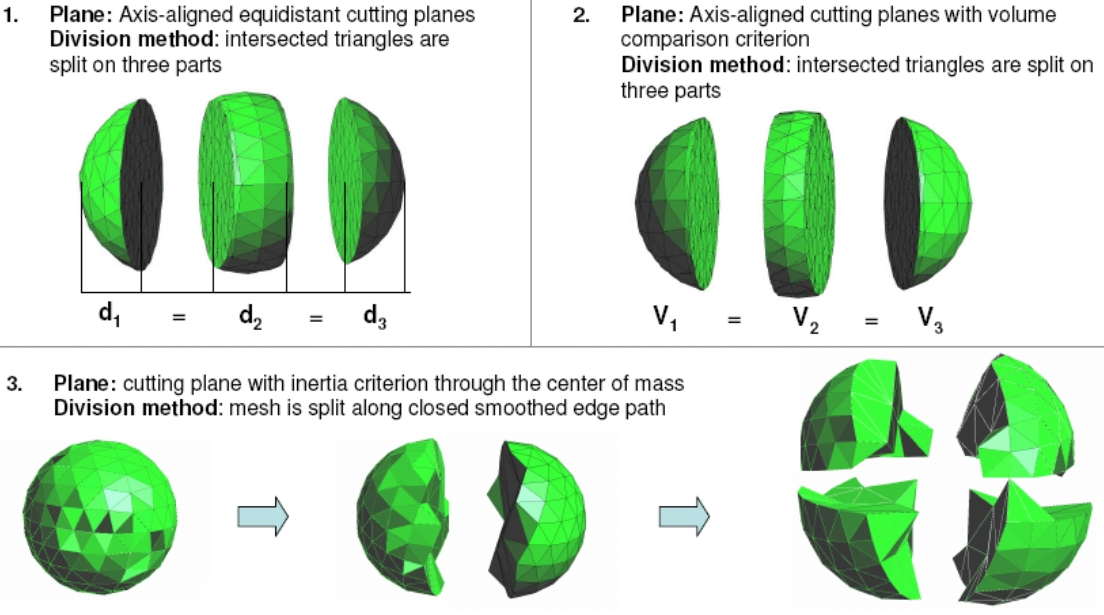
\includegraphics[width=0.9\textwidth]{imagem2}
     \caption{As 3 formas de particionar. 1 - planos equidistantes. 2 - volume dos subdomínios iguais. 3 - centro de massa \cite{bib:Ivanov06}.}
     \label{fig:imagem2}
 \end{figure}

Uma solução parecida é a de \cite{bib:Lammer00}, que traçam o plano de corte da mesma maneira porém em duas dimensões. Esse eixo é usado para dividir o domínio recursivamente. A partir do eixo, uma aresta é formada, e os valores nos seus pontos extremos são interpolados dos valores dados como entrada. Quando o número de subdomínios for igual ao número de processadores, uma malha de Delaunay é gerada em cada interior.

\section{Particionamento Baseado em \textit{Octree}/\textit{Quadtree}}

Em \cite{bib:deCougny99}, a entrada do algoritmo é o contorno de um objeto. Cada processador terá parte de uma \textit{octree} distribuída, criando planos de corte do domínio. A malha das células internas é gerada concorrentemente com \textit{templates}. A região entre o contorno e as células internas é preenchida por uma técnica de avanço de fronteira, onde são gerados os elementos internos a uma região delimitada pelos planos de corte. Por último é feita a conexão das malhas dos dois lados de cada plano e suas intersecções.

Na técnica de \cite{bib:Lohner01}, é gerada uma \textit{octree} grosseira com relação ao contorno dado como entrada. Então, as células que contêm a parte da fronteira que gerará os menores elementos são identificadas. Assim, partes da malha, correspondentes a cada célula, são geradas simultaneamente por avanço de fronteira, de maneira que cada parte da malha gerada não possa cruzar as extremidades da célula que a contém. Então, cada octante sofre um pequeno deslocamento na diagonal com o intuito de gerar mais elementos. Esse deslocamento elimina quase todas as faces entre duas ou mais células e diminui o tamanho da fronteira para o próximo passo. Assim, a nova fronteira é encontrada, uma nova \textit{octree} é construída para ela, e o procedimento é repetido, até que não seja mais possível gerar malha.

\cite{bib:Larwood03} apresentam uma técnica de decomposição de domínio que tem como entrada uma triangulação de borda. Para saber quais subdomínios devem ser divididos, o autor usa um critério baseado na quantidade de faces por subdomínio. A decomposição é feita recursivamente usando uma \textit{octree} caso seja tridimensional ou uma \textit{quadtree} caso seja bidimensional, verificando sempre se o número de faces de um subdomínio é menor do que o limite estipulado, e, enquanto a verificação for falsa, a decomposição irá ocorrer. A quantidade máxima de subdivisões está limitada por uma constante maior que o número de processadores disponíveis, isso evita a criação excessiva de partições e permite que um processador possa receber mais de uma tarefa ao longo da execução.

Para evitar a criação de elementos ruins é feita uma verificação no corte, que é baseada no ângulo do vetor normal do plano de corte com a normal dos triângulos, de tal forma que o plano de corte não possa passar por triângulos com ângulo menor do que uma tolerância. Como o plano de corte é baseado na \textit{octree} se tridimensional ou na \textit{quadtree} se bidimensional, será necessário um deslocamento na mesma caso a verificação do corte falhe. A imagem~\ref{fig:imagem3} mostra um exemplo onde alguns planos de corte falham nos testes.

 \begin{figure}[htbp]
     \centering
     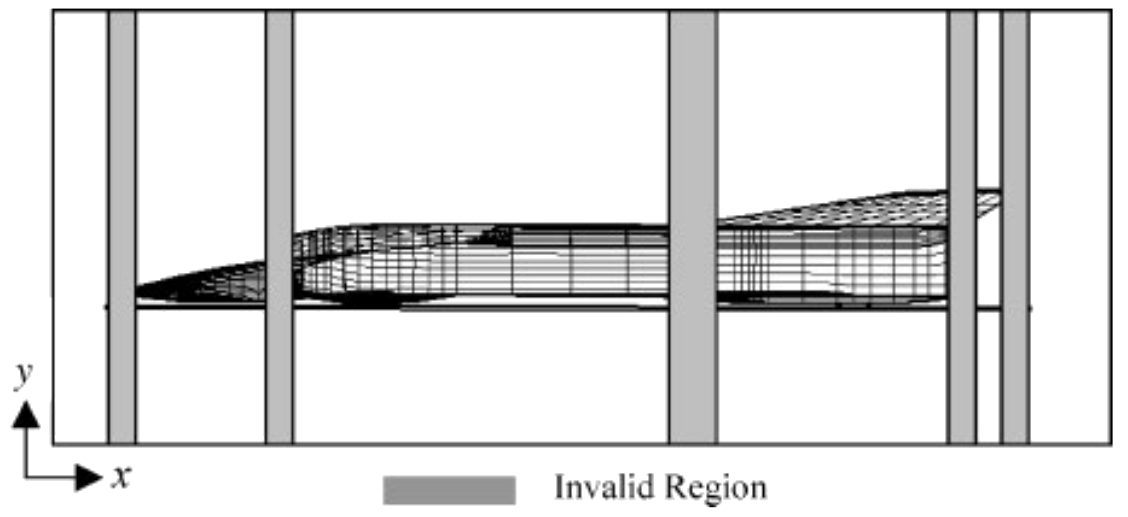
\includegraphics[width=0.9\textwidth]{imagem3}
     \caption{Regiões de corte invalidas em cinza \cite{bib:Larwood03}.}
     \label{fig:imagem3}
 \end{figure}

\section{Particionamento Baseado no Eixo Mediano}

O Eixo Mediano(EM) é uma maneira de descrever a forma de um objecto. O EM é utilizado para garantir uma decomposição de domínio com separadores que formam bons ângulos entre eles e as bordas. 

Em \cite{bib:Leonidas06} apresenta uma técnica bidimensional que utiliza a triangularização de Delaunay por divisão e conquista para um conjunto de pontos dados como entrada. Primeiramente é feito uma triangulação da borda, essa triangulação é utilizada para a geração de um grafo ponderado, onde o peso das arestas serão iguais ao raio da circunferência circunscrita do triângulo que contém essa aresta. Em seguida é feito uma contração dessa grafo. 

 \begin{figure}[htbp]
     \centering
     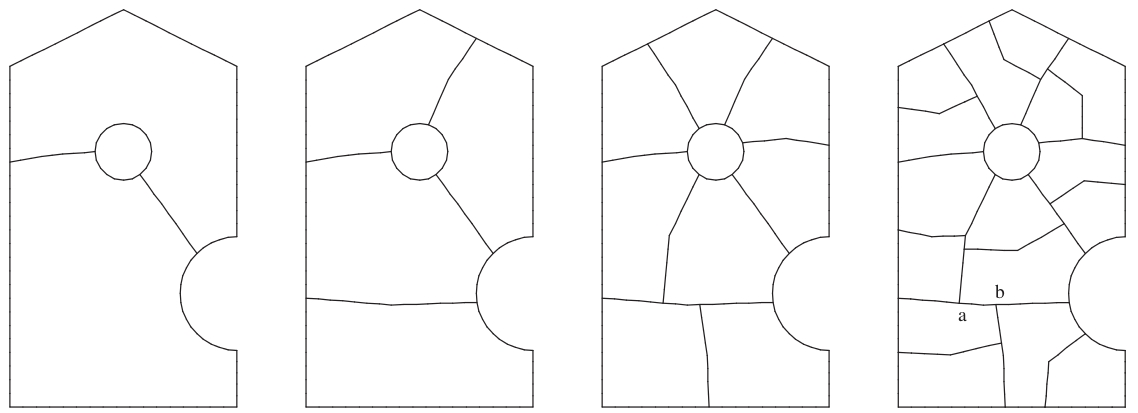
\includegraphics[width=0.9\textwidth]{imagem4}
     \caption{Partições em 2,4,8 e 16. \cite{bib:Leonidas06}.}
     \label{fig:imagem4}
 \end{figure}

Através do grafo formado os planos de corte serão posicionados e os subdomínios formados. A figura~\ref{fig:imagem4} mostra o resultado de particionamentos para quantidades diferentes de subdomínios. Após isso a geração da malha interna poderá ser realizada.

\section{Particionamento Baseado em \textit{Bounding Box}}

Em \cite{bib:Glut08}, é apresenta uma técnica para malhas tridimensionais. Essa é uma abordagem baseada na decomposição geométrica onde a entrada é uma malha de superfície. Aqui é apresentado duas técnicas baseadas na \textit{bounding box} gerada a partir da entrada.

A seleção do separador do domínio deve garantir um custo de corte baixo, ou seja, encontrar e posicionar o plano de corte não pode ter um custo computacional alto. Além disse deve garantir um bom balanceamento de carga e minimizar os elementos conectados por múltiplos subdomínios.

A primeira técnica é baseada na malha de superfície. Para o plano de corte ser criado é preciso a localização do contorno da malha de superfície e do separador. O contorno é então projetado no separador usando uma função 2D de controle espacial baseada no tamanho das arestas. Ver figura~\ref{fig:imagem5}.

 \begin{figure}[htbp]
     \centering
     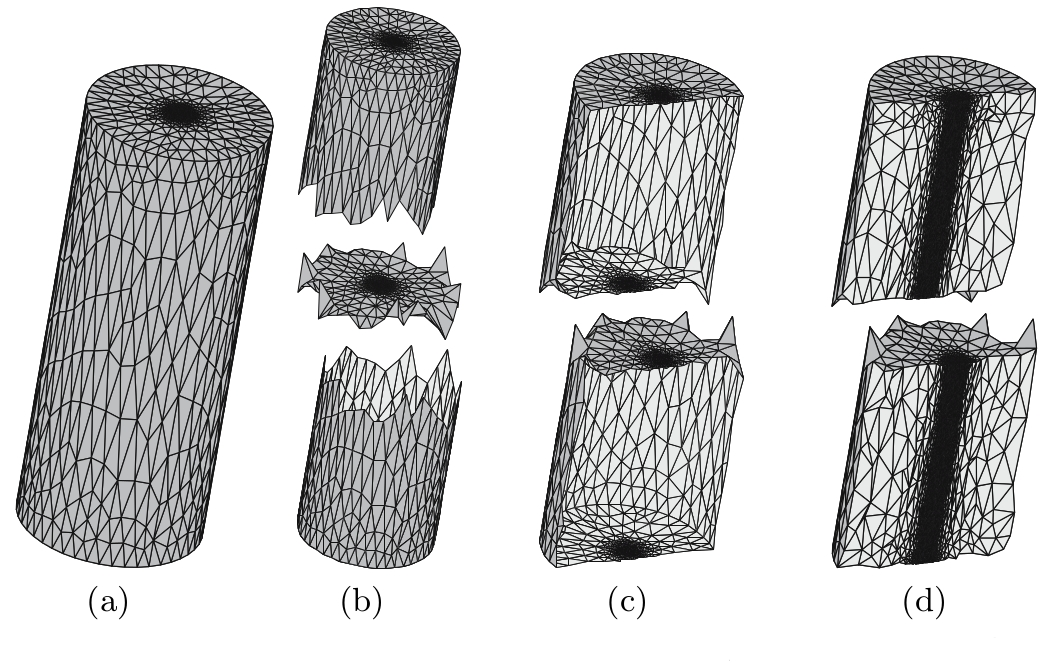
\includegraphics[width=0.9\textwidth]{imagem5}
     \caption{Passos da técnica baseado na malha de superfície. (a) malha de superfície; (b) corte; (c) seção transversal; (d) malha final. \cite{bib:Glut08}.}
     \label{fig:imagem5}
 \end{figure}

A segunda técnica se baseia numa malha volumétrica grosseira. Primeiramente é feito a geração de uma malha 3D grosseira utilizando alguma função de controle espacial. O posicionamento do plano de corte é feito parecido com a técnica anterior sendo que será utilizado a malha volumétrica para a função espacial. Ver figura~\ref{fig:imagem6}.

 \begin{figure}[htbp]
     \centering
     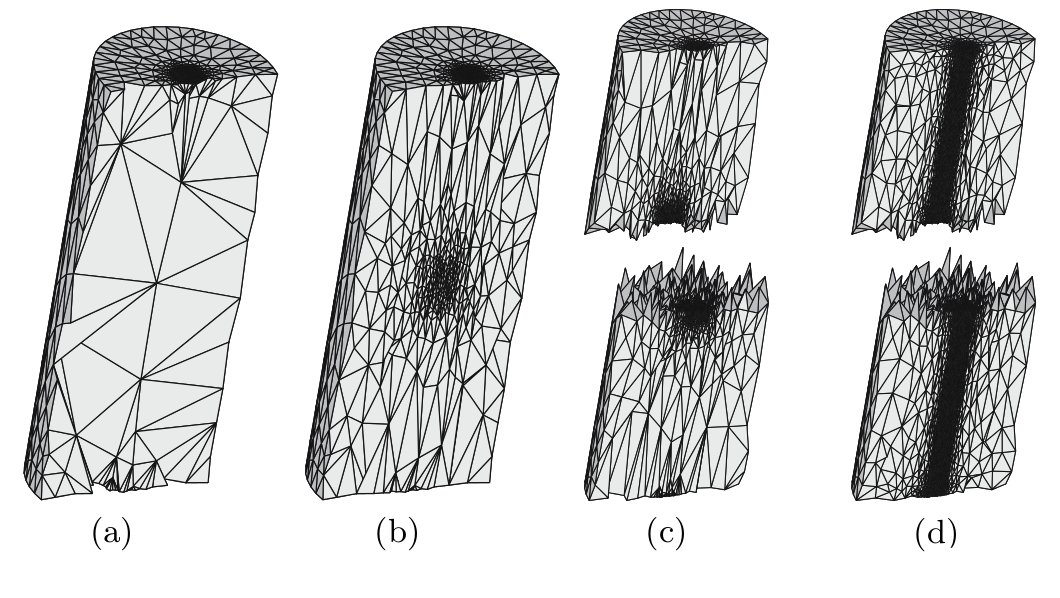
\includegraphics[width=0.9\textwidth]{imagem6}
     \caption{Passos da técnica se basea na malha volumétrica grosseira. (a) malha volumétrica grosseira; (b) refinamento da seção transversal; (c) seção transversal; (d) malha final. \cite{bib:Glut08}.}
     \label{fig:imagem6}
 \end{figure}

Essa técnica depende muito da geometria da entrada já que é utilizada informações da \textit{bounding box} da entrada. Isso afeta diretamente a criação dos plano de corte e por consequência a malha gerada ao final.

